\documentclass{beamer}

%\usepackage[utf8]{inputenc}
\usepackage[T1]{fontenc}
\usepackage{fontspec}
\usepackage[brazil]{babel}
\usepackage{listings}
\usepackage{graphicx}
\usepackage{color}
\definecolor{editorGray}{rgb}{0.95, 0.95, 0.95}
\definecolor{editorOcher}{rgb}{1, 0.5, 0} % #FF7F00 -> rgb(239, 169, 0)
\definecolor{editorGreen}{rgb}{0, 0.5, 0} % #007C00 -> rgb(0, 124, 0)
\usetheme[outer/progressbar=foot]{Metropolis}
\setsansfont[BoldFont={Source Sans Pro Semibold},Numbers={OldStyle}]{Source Sans Pro}

%\makeatletter
%\def\verbatim@font{\ttfamily}
%\makeatother

\lstset{%
    % Basic design
    backgroundcolor=\color{editorGray},
    basicstyle={\scriptsize\ttfamily},   
	%basicstyle={\scriptsize},   
    frame=l,
    % Line numbers
    xleftmargin={0.75cm},
   % numbers=left,
    stepnumber=1,
    firstnumber=1,
    numberfirstline=true,
    % Code design   
    keywordstyle=\color{blue}\bfseries,
    commentstyle=\color{darkgray}\ttfamily,
    ndkeywordstyle=\color{editorGreen}\bfseries,
    stringstyle=\color{editorOcher},
    % Code
    language=csh,
    alsodigit={.:;},
    tabsize=2,
    showtabs=false,
    showspaces=false,
    showstringspaces=false,
    extendedchars=true,
    breaklines=true,
    morekeywords={
    	abstract, event, new, struct,
    	as, explicit, null, switch,
    	base, extern, object, this,
    	bool, false, operator, throw,
    	break, finally, out, true,
    	byte, fixed, override, try,
    	case, float, params, typeof,
    	catch, for, private, uint,
    	char, foreach, protected, ulong,
    	checked, goto, public, unchecked,
    	class, if, readonly, unsafe,
    	const, implicit, ref, ushort,
    	continue, in, return, using,
    	decimal, int, sbyte, virtual,
    	default, interface, sealed, volatile,
    	delegate, internal, short, void,
    	do, sizeof, while,
    	double, lock, stackalloc,
    	else, long, static,
    	enum, namespace, string
    },
    literate={ç}{{\c{c}}}1 {é}{{\'e}}1 {á}{{\'a}}1 {ã}{{\~a}}1 {ó}{{\'o}}1 {í}{{\'i}}1
}

\begin{document}
\title{Programação Básica em C\# para Unity - MonoBehaviours}   
\author{Bruno dos Santos de Araújo, MSc} 
\date{\today} 

%\AtBeginSection[]
%{
%  \begin{frame}
%  \frametitle{Sumário}
%  \tableofcontents[currentsection]
%  \end{frame}
%}

\frame{\titlepage} 

\frame{\frametitle{Sumário}\tableofcontents} 

\section{Introdução}

\begin{frame}[fragile]{Introdução}
	\begin{itemize}
		\item Este treinamento tem os seguintes objetivos:
		\begin{itemize}
			\item Entender o conceito de \verb|game loop| e como se aplica ao Unity;
			\item Mostrar a estrutura básica do tipo de script mais comum no Unity: \verb|MonoBehaviour|;
			\item Implementar uma versão simples porém funcional do jogo Breakout (também conhecido como Arkanoid).
		\end{itemize}
		\item Existem diversas abordagens possíveis para os problemas que iremos resolver, neste treinamento utilizaremos as abordagens mais simples e didáticas e não necessariamente as mais eficientes.
	\end{itemize}
\end{frame}

\section{Game loop}

\begin{frame}[fragile]{Game loop}
	\begin{itemize}
		\item Quase todos os jogos utilizam um algoritmo chamado \verb|game loop|, que basicamente possui 3 funções:
		\begin{itemize}
			\item Ler e processar a entrada do usuário
			\item Atualizar o estado interno do jogo
			\item Desenhar a tela
		\end{itemize}
		\item O número de vezes que esse algoritmo é executado por segundo determina a taxa de \textbf{quadros por segundo} do jogo, ou \textbf{FPS} (frames per second)
		\begin{itemize}
			\item 30 FPS: a cada ~33ms
			\item 60 FPS: a cada ~16ms
		\end{itemize}
	\end{itemize}
\end{frame}

\begin{frame}[fragile]{Game loop}
	\begin{itemize}
		\item Visualização do algoritmo:
	\end{itemize}		
	\begin{lstlisting}
while(gameIsRunnning) {
	readInput();
	update();
	render();
}
\end{lstlisting}
	\begin{itemize}
		\item \verb|readInput()|: lê a entrada do usuário
		\item \verb|update()|: atualiza o estado interno do jogo
		\item \verb|render()|: desenha a tela
	\end{itemize}
\end{frame}

\begin{frame}[fragile]{Game loop}
%	\begin{itemize}
%		\item Visualização do algoritmo:
%	\end{itemize}		
%	
%	\begin{lstlisting}
%while(gameIsRunnning) {
%	readInput();
%	update();
%	render();
%}
%	\end{lstlisting}
	\begin{itemize}
		\item Ao implementar código de gameplay no Unity, precisamos sempre implementar os equivalentes a \verb|readInput()| e \verb|update()| dentro de uma subclasse de \verb|MonoBehaviour|.
		\begin{itemize}
			\item \verb|render()| é implementada via shaders; mesmo que você não escreva nenhum, o Unity utiliza shaders padrão
		\end{itemize}
	\begin{itemize}
		\item Boa referência sobre o assunto: \url{https://gameprogrammingpatterns.com/game-loop.html}
	\end{itemize}
	\end{itemize}
\end{frame}

\section{Estrutura de um MonoBehaviour}

\begin{frame}[fragile]{Estrutura de um MonoBehaviour}
	\begin{itemize}
		\item \verb|MonoBehaviour| é a classe da qual se deriva a maioria dos componentes dentro do Unity.
		\item Ao criarmos um novo \verb|MonoBehaviour|, seja diretamente como componente num GameObject ou na hierarquia, nos deparamos com o seguinte código:		
	\end{itemize}
	\begin{lstlisting}
public class NewBehaviourScript : MonoBehaviour
{
	void Start()
	{
	}
	
	void Update()
	{	
	}
}	
	\end{lstlisting}
	\begin{itemize}
		\item Podemos observar duas funções que foram criadas por padrão: \verb|Start()| e \verb|Update()|.
	\end{itemize}
\end{frame}

\begin{frame}[fragile]{Estrutura de um MonoBehaviour}
	\begin{itemize}
		\item \verb|Start()|: esta função é chamada uma vez assim que o script é ativado pela primeira vez, sempre antes da primeira chamada a \verb|Update()|.
		\begin{itemize}
			\item Normalmente utilizada para inicializar quaisquer variáveis e chamar funções de inicialização.
			\item Devido a ser executado só na ativação do script, pode ser utilizada para atrasar a inicialização para o momento que seja mais conveniente.
		\end{itemize}
	\end{itemize}
	\begin{lstlisting}
private void Start()
{
	maxHp = 10;
	transform.position = GetInitialPosition();		
}
\end{lstlisting}
\end{frame}


\begin{frame}[fragile]{Estrutura de um MonoBehaviour}
	\begin{itemize}
		\item \verb|Update()|: esta função é chamada a cada quadro quando o script está ativado, e é utilizada para atualizar o estado interno do componente. 
		\begin{itemize}
			\item No caso de ser um objeto controlável pelo jogador, também é onde se leem as entradas (teclas, botões, etc);
			\item O tempo entre chamadas é aproximadamente o mesmo e pode variar de acordo com a quantidade de objetos na cena.
		\end{itemize}
	\end{itemize}
	\begin{lstlisting}
private void Update()
{
	// Update position at each frame
	transform.position += velocity * Time.deltaTime;
}
\end{lstlisting}
\begin{itemize}
	\item Outras funções comumente utilizadas seguem nos próximos slides.
\end{itemize}
\end{frame}

\begin{frame}[fragile]{Estrutura de um MonoBehaviour}
	\begin{itemize}
		\item \verb|Awake()|: é chamada uma única vez no ato da criação do GameObject, sempre antes de \verb|Start()|;
		\begin{itemize}
			\item Normalmente utilizada para obter referências a componentes locais do GameObject e para instruções que precisam ser executadas sempre antes de \verb|Start()|.
			\item Se o objeto não estiver ativado na inicialização da cena, será chamada na primeira vez que o objeto for ativado.
			\item Se o objeto estiver ativo mas não o script, \verb|Awake()| será chamada.
		\end{itemize}

	\end{itemize}
	\begin{lstlisting}
private void Awake()
{
	rigidBody = GetComponent<Rigidbody>();
	animator = GetComponent<Animator>();
}
	\end{lstlisting}
\end{frame}

\begin{frame}[fragile]{Estrutura de um MonoBehaviour}
	\begin{itemize}
		\item \verb|FixedUpdate()|: semelhante a \verb|Update()| mas é chamada em tempos fixos a cada passo da Física, que por padrão é 20ms;
		\begin{itemize}
			\item Utilizada principalmente quando se utilizam funções que agem na física do GameObject.
		\end{itemize}
	\end{itemize}
	\begin{lstlisting}
private void FixedUpdate()
{
	if(Input.GetKey(KeyCode.RightArrow))
	{
		rigidbody.AddForce(Vector3.right * forceAmount);
	}
}
	\end{lstlisting}
\end{frame}


\begin{frame}[fragile]{Estrutura de um MonoBehaviour}
	\begin{itemize}
		\item \verb|OnEnable()| e \verb|OnDisable()|: chamadas na ativação e desativação do GameObject, respectivamente;
		\item Permitem separar a inicialização de maneira mais granular, e também executar algum código na desativação do objeto.
	\end{itemize}
	
	\begin{lstlisting}
// assume the game has a minimap showing the enemies
private void OnEnable()
{
	AddToMinimap();
}

private void OnDisable()
{
	RemoveFromMinimap();
}
	\end{lstlisting}
\end{frame}


\begin{frame}[fragile]{Estrutura de um MonoBehaviour}
	\begin{itemize}
		\item \verb|OnDestroy()|: chamada quando o objeto é destruído, seja quando a cena é descarregada ou usando \verb|Destroy()| diretamente.
		\begin{itemize}
			\item Menos comumente utilizada, mas útil pra quaisquer tarefas de limpeza quando o objeto é destruído.
		\end{itemize}
	\end{itemize}
	\begin{lstlisting}
private void Destroy()
{
	RemoveFromEnemyList();
}
	\end{lstlisting}
\end{frame}

\begin{frame}[fragile]{Exemplo da ordem de execução dos scripts}
	
\begin{columns}
\column{0.5\textwidth}
\begin{lstlisting}
private void Awake() {
	Debug.Log("Awake()");
}

private void Start() {
	Debug.Log("Start()");
}

private void OnEnable() {
	Debug.Log("OnEnable()");
}
\end{lstlisting}

\column{0.5\textwidth}
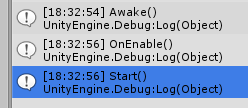
\includegraphics{executionorder.png}
\end{columns}
	
\end{frame}


\end{document}

